\section{Aula 6.4 - Multiplexação por divisão no tempo II}

Nessa aula ficamos a par do padrão internacional T-1.

\subsection{O padrão T-1}

Esse padrão foi desenvolvido pela Bell Labs, empresa americana, e é um exemplo prático de como o TDM é aplicado na realidade.
a composição da hierarquia T-1 é dada da seguinte maneira:
\\\\
\textbf{24 canais de voz -> para cada canal um modulador PCM -> mux}
\\
A largura de banda de cada canal é de \textit{4Khz} e a taxa de bits que é enviada é de \textit{64kpbs}

E o modulador PCM amostra a uma taxa de \textit{8k amostras/s} e \textit{8 bits para etapa de quantização}

E por fim cada linha fornece \textit{8 bits+1 de sincronismo} para compor o frame

E a taxa de frames é de \textit{8k frames/s}

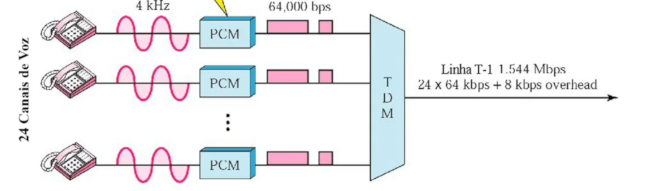
\includegraphics[width=0.7\textwidth]{../assets/tdm.png}

\subsection{A hierarquia TDM}

E para terminar essa seção a saída do mux é cascateada em outro mux segundo uma sequência de multiplicadores até que chegue no nível mais elevado que em tese
seriam as taxas de enlace mais rápidas fornecidas pelo sistema. Abaixo uma comparação entre modelo Europeu e Americano.

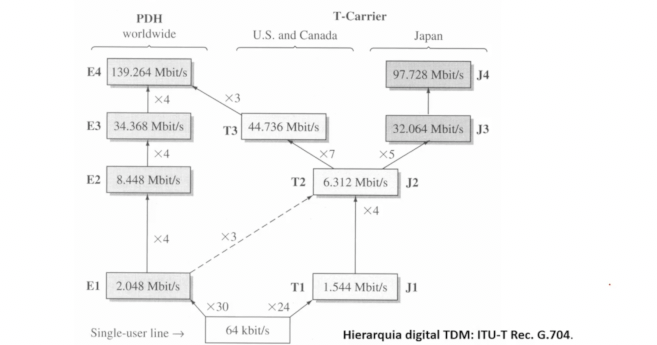
\includegraphics[width=0.8\textwidth]{../assets/hire.png}

Note que os números na saída dos blocos são o número de cascatas que ocorrem antes de chegar no próximo nível da hierarquia, note ainda que quanto maior o número a
direita da letra E4 por exemplo indica uma maior taxa de enlace e note que há uma comunicação entre o bloco branco, USA, cinza escuro, Japão e o que sobrou Europa num
determinado nível da hierarquia
